\section{Arquitectura del Sistema}

La arquitectura del sistema se basa por completo en el uso de \textit{Next.js}, un framework de \textit{React} que permite la creación de aplicaciones web, con la funcionalidad clave de un backend integrado. Desde la versión 13 de \textit{Next.js} se introdujo el concepto de \textbf{App Router}, que crea las rutas de la web en base a la organización de las carpetas dentro del proyecto. Junto a esto, se introdujeron los \textbf{Route Handlers}, que permiten la creación de endpoints API REST de la misma manera, creando un backend integrado que hace de intermediario entre el cliente y los servicios externos. De esta manera, se consigue una arquitectura notablemente más simplificada, además de segura, ya que se puede controlar la exposición de datos sensibles al cliente.

Otra caracterísitica muy útil de \textit{Next.js}, son los \textbf{Server Components}, que permiten renderizar componentes en el servidor en lugar del cliente. Solo aquellos componentes que sean necesarios serán enviados y ejecutados en el cliente, mejorando el rendimiento y la seguridad. Estos componentes pueden realizar llamadas a los endpoints proporcionados por los \textit{Route Handlers}, recreando los roles de un sistema cliente-servidor tradicional. En el diagrama \ref{fig:arquitectura_sistema} se pueden ver representadas estas interacciones.

\begin{figure}[H]
    \centering
    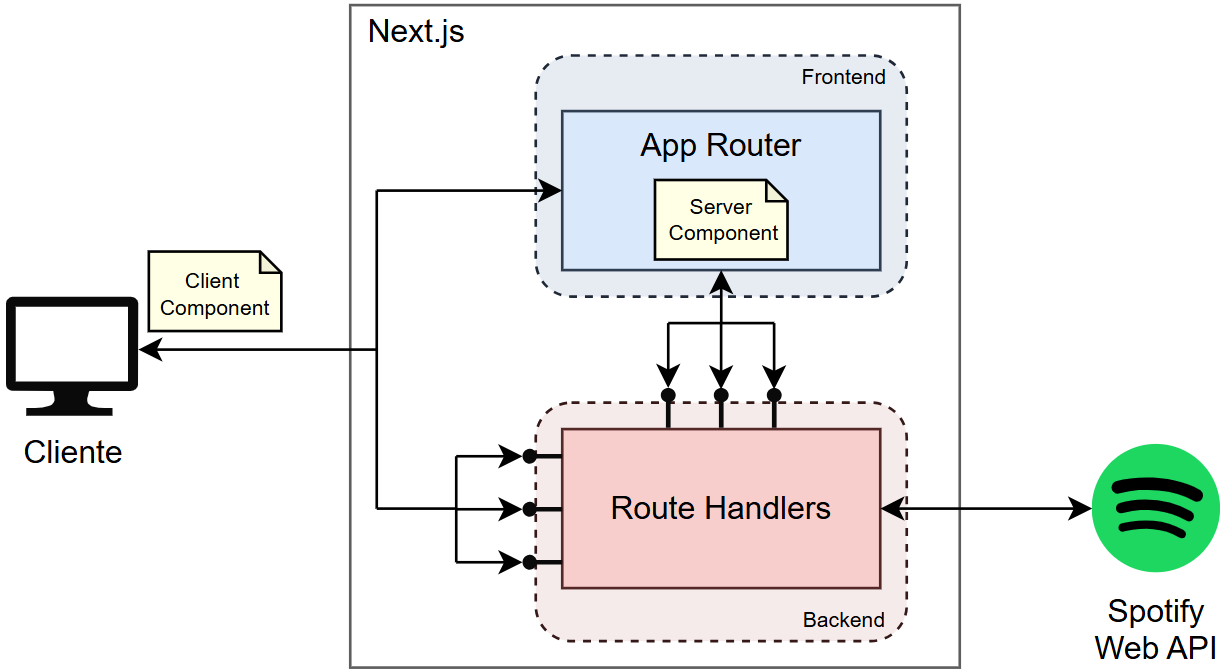
\includegraphics[width=0.85\textwidth]{figures/arquitectura_sistema.png}
    \caption{Diagrama de la arquitectura del sistema haciendo uso de \textit{Next.js}.}
    \label{fig:arquitectura_sistema}
\end{figure}

\subsection{Rutas del Frontend}

Usando el \textit{App Router}, las rutas del frontend se organizan en la carpeta \texttt{app/}, donde cada subcarpeta representa una ruta específica en la web. Dentro de cada carpeta se pueden encontrar archivos específicos que siguen una convención de nombres, y que definen su función. Las más importantes son:

\begin{itemize}
    \item \texttt{layout.tsx}: Define el diseño compartido de los componentes que se encuentran anidados en las subcarpetas interiores.
    \item \texttt{page.tsx}: Contiene el contenido principal de una ruta específica. Representa la página renderizada cuando el usuario accede a esa ruta. \textbf{Para que una página sea accesible, debe existir un archivo \texttt{page.tsx} en la carpeta correspondiente}.
    \item \texttt{loading.tsx}: Muestra un indicador de carga mientras se obtienen datos o se renderizan componentes en una página.
    \item \texttt{error.tsx}: Gestiona errores específicos de una página, mostrando mensajes o interfaces para el usuario en caso de fallos.
\end{itemize}

En el caso de este proyecto, la jerarquía de carpetas que genera las páginas routeables de la web es la siguiente:

\begin{verbatim}
    app/
    ├── home/
    │   └── page.tsx (Ruta: /home)
    ├── stats/
    │   └── page.tsx (Ruta: /stats)
    └── page.tsx (Ruta: /)
\end{verbatim}

La ruta \texttt{/} (raíz) es la página principal, en donde el usuario puede iniciar sesión. Las rutas \texttt{/home} y \texttt{/stats} representan las páginas de estadísticas básicas y estadísticas avanzadas, respectivamente. En cada caso, el archivo \texttt{page.tsx} define el contenido principal de la página y es posible añadir otros archivos como \texttt{layout.tsx}, \texttt{loading.tsx} o \texttt{error.tsx} para mejorar la experiencia del usuario.

\subsection{Endpoints del Backend}

En el caso de la creación de endpoints mediante los \textit{Route Handlers}, la estructura de carpetas es similar a la de las rutas del frontend, pero con la diferencia de que cada subcarpeta dentro de \texttt{app/api/} contiene un archivo \texttt{route.ts} que define el comportamiento del endpoint asociado. \textbf{Para que un endpoint sea accesible, debe existir un archivo \texttt{route.ts} en la carpeta correspondiente}.

La estructura de carpetas para los endpoints de este proyecto es la siguiente:

\newpage

\begin{verbatim}
    app/
    └── api/
        ├── auth/
        │   ├── callback/route.ts
        │   ├── login/route.ts
        │   └── logout/route.ts
        ├── home/
        │   ├── recently-played/route.ts
        │   ├── top-artists/route.ts
        │   ├── top-genres/route.ts
        │   ├── top-tracks/route.ts
        │   └── user-profile/route.ts
        └── stats/
            ├── estaciones-musicales/route.ts
            ├── hall-of-fame/route.ts
            ├── huella-del-dia/route.ts
            ├── indice-de-resonancia/route.ts
            ├── la-bitacora/route.ts
            └── tus-decadas/route.ts
\end{verbatim}

Los endpoints en \texttt{/api/auth/} gestionan el incio de sesión del usuario, mientras que los de \texttt{/api/home/} y \texttt{/api/stats/} se encargan de obtener y procesar los datos necesarios para las estadísiticas. El contenido del fichero \texttt{route.ts} sigue una convención concreta que \textit{Next.js} reconoce y utiliza para gestionar las peticiones, la cual se explicará con más detalle en el capítulo de \nameref{ch:implementacion}.

\section{Diagrama de Componentes de React}

Los componentes en \textit{React} son las piezas fundamentales para construir interfaces de usuario. Cada componente puede ser reutilizable, contener su propio estado y lógica, y ser combinado con otros para formar estructuras más complejas. Además, en \textit{React}, las interfaces se suelen diseñar en forma de jerarquías de componentes, en las que los componentes ``padre'' organizan y controlan el comportamiento y la presentación de los componentes ``hijo''. Esta organización jerárquica facilita el mantenimiento y la escalabilidad del código, ya que cada componente tiene una responsabilidad definida.

En este proyecto, se ha creado una jerarquía de componentes (diagrama \ref{fig:componentes_react}) que refleja las diferentes funcionalidades de la aplicación. A la hora de construir la web, \textit{Next.js} y \textit{React} se encargan de anidar los componentes necesarios y renderizarlos, o enviarlos al cliente, según sea necesario.

\begin{figure}[H]
    \centering
    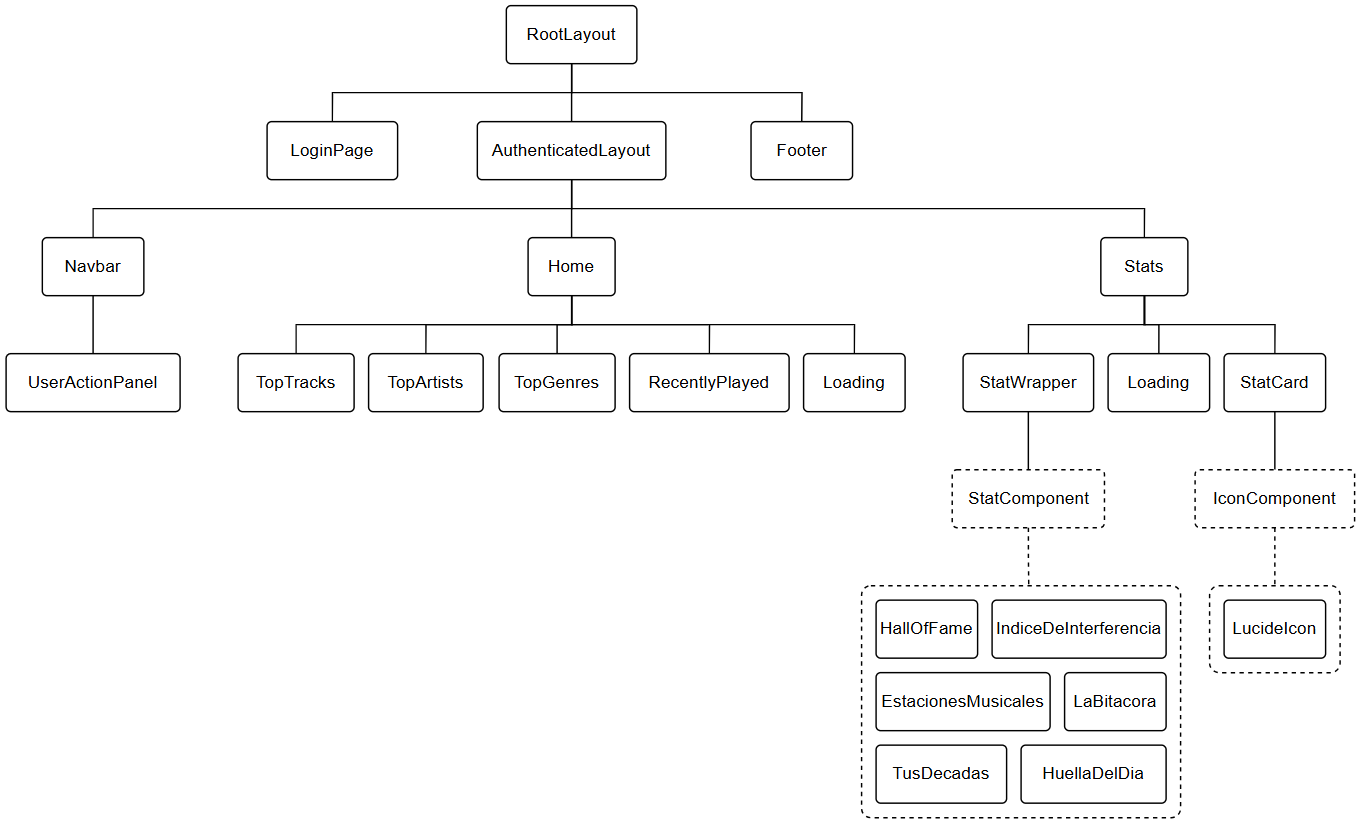
\includegraphics[width=\textwidth]{figures/componentes_react.png}
    \caption{Diagrama de la jerarquía de componentes de React creados en el proyecto.}
    \label{fig:componentes_react}
\end{figure}

La mayoría de los componentes están definidos de manera explícita y son renderizados cuando se llegue a una ruta en concreto, pero hay otros componentes que se cargan dinámicamente, es decir, el contenido que aparece en su lugar puede variar en función de las acciones del usuario o del contexto del componente. Se podría considerar que el componente hijo temporal, se ``transforma'' en otro que toma su lugar. En este proyecto, se han definido dos componentes que se comportan así:

\begin{itemize}
    \item \textbf{StatComponent}: Se utiliza para mostrar una de las seis estadísticas disponibles, cada una siendo un componente autocontenido. Dependiendo de la selección del usuario, se cargará uno de estos subcomponentes en el lugar correspondiente. También se puede inferir que solo se podrá mostrar una estadística a la vez.
    \item \textbf{IconComponent}: Está asociado con los iconos representativos de cada estadística, que se muestran en las tarjetas (\texttt{StatCard}) que el usuario puede clicar para verla. Utiliza el paquete \texttt{LucideIcon} para cargar diferentes iconos, ya que, en este paquete, cada icono es representado como un componente de \textit{React}.
\end{itemize}

Con este diseño, en especial con el componente \texttt{StatComponent}, se reduce la cantidad de código a renderizar y enviar al cliente, ya que solamente se cargará la estadística necesaria y cuando el usuario lo solicite. Además, en el desarrollo se puede encapsular toda la lógica necesaria para cada estadística en un único componente, facilitando la incorporación de nuevas estadísticas, si hace falta.


% TODO: Queda esta sección por completar
\section{Interfaz de Usuario}

\subsection{Principios de Diseño}
Basado en el lenguaje de diseño de Spotify
https://developer.spotify.com/documentation/design

\subsection{Distribución de la Interfaz}
Navegación
distribución de contenido
describir páginas principales
organizacion de datos en la interfaz para que fuese comprensible

\subsection{Responsividad}
Responsivo: se ajusta a diferentes tamaños de pantalla mientras lo mueves
(Adaptativo: se establece cómo se debería de ver en diferentes tamaños de pantalla. Hace un salto cuando cambia de tamaño)

Tailwind

\subsection{Gráficos y Visualización de Datos}
Cómo se presentan?
Qué tipos de gráficos?
Cómo interactúa el usuario?
% TODO: --------------------------------



% TODO: Preguntar si dejar aquí o mover a anexo. Aquí no sé qué explicar.
\section{Diagramas de Secuencia}

\begin{figure}[H]
    \centering
    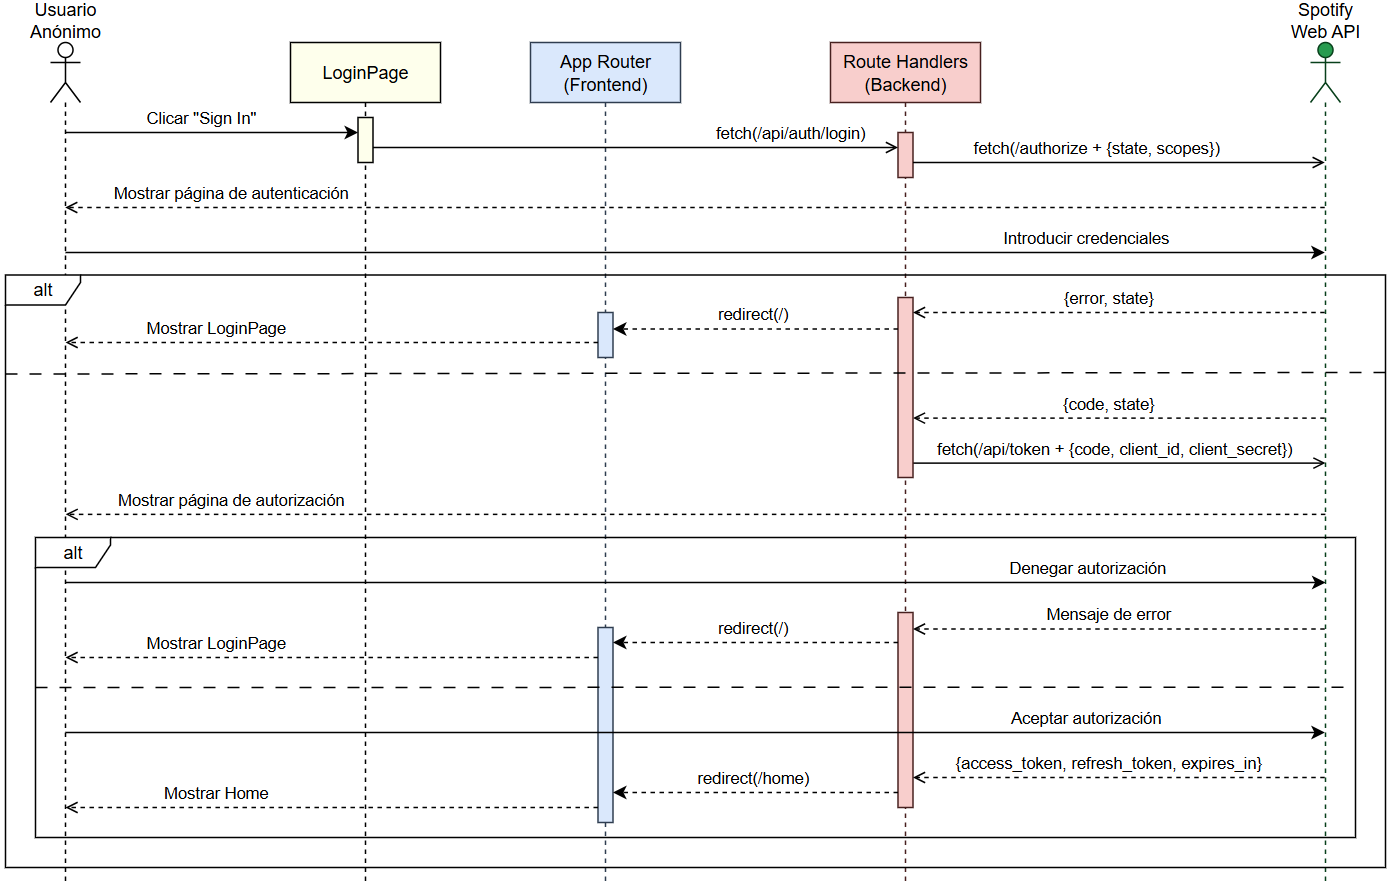
\includegraphics[width=\textwidth]{figures/diagramas_secuencia/ds_iniciar_sesion.png}
    \caption{Diagrama de secuencia: Iniciar Sesión.}
    \label{fig:ds_iniciar_sesion}
\end{figure}

\begin{figure}[H]
    \centering
    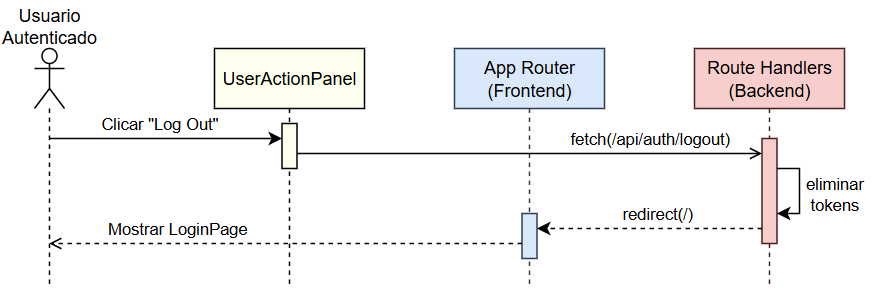
\includegraphics[width=0.85\textwidth]{figures/diagramas_secuencia/ds_cerrar_sesion.png}
    \caption{Diagrama de secuencia: Cerrar Sesión.}
    \label{fig:ds_cerrar_sesion}
\end{figure}

\begin{figure}[H]
    \centering
    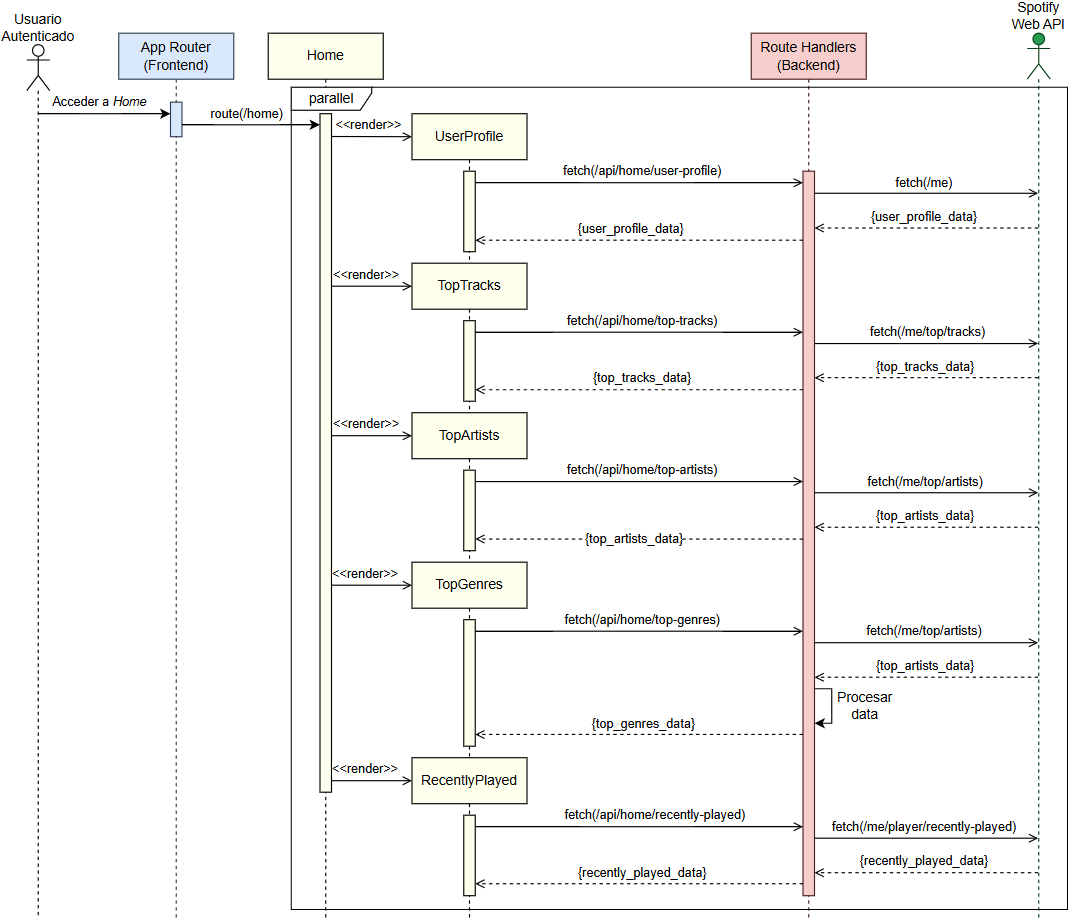
\includegraphics[width=\textwidth]{figures/diagramas_secuencia/ds_acceder_home.png}
    \caption{Diagrama de secuencia: Acceder a \textit{Home}.}
    \label{fig:ds_acceder_home}
\end{figure}

\begin{figure}[H]
    \centering
    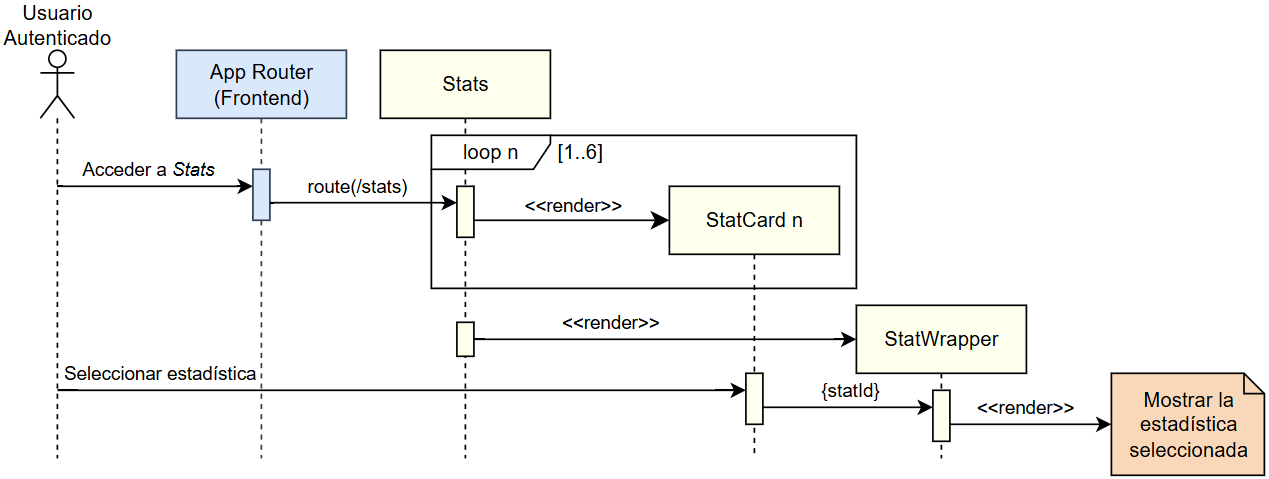
\includegraphics[width=0.9\textwidth]{figures/diagramas_secuencia/ds_acceder_stats.png}
    \caption{Diagrama de secuencia: Acceder a \textit{Stats}.}
    \label{fig:ds_acceder_stats}
\end{figure}

\begin{figure}[H]
    \centering
    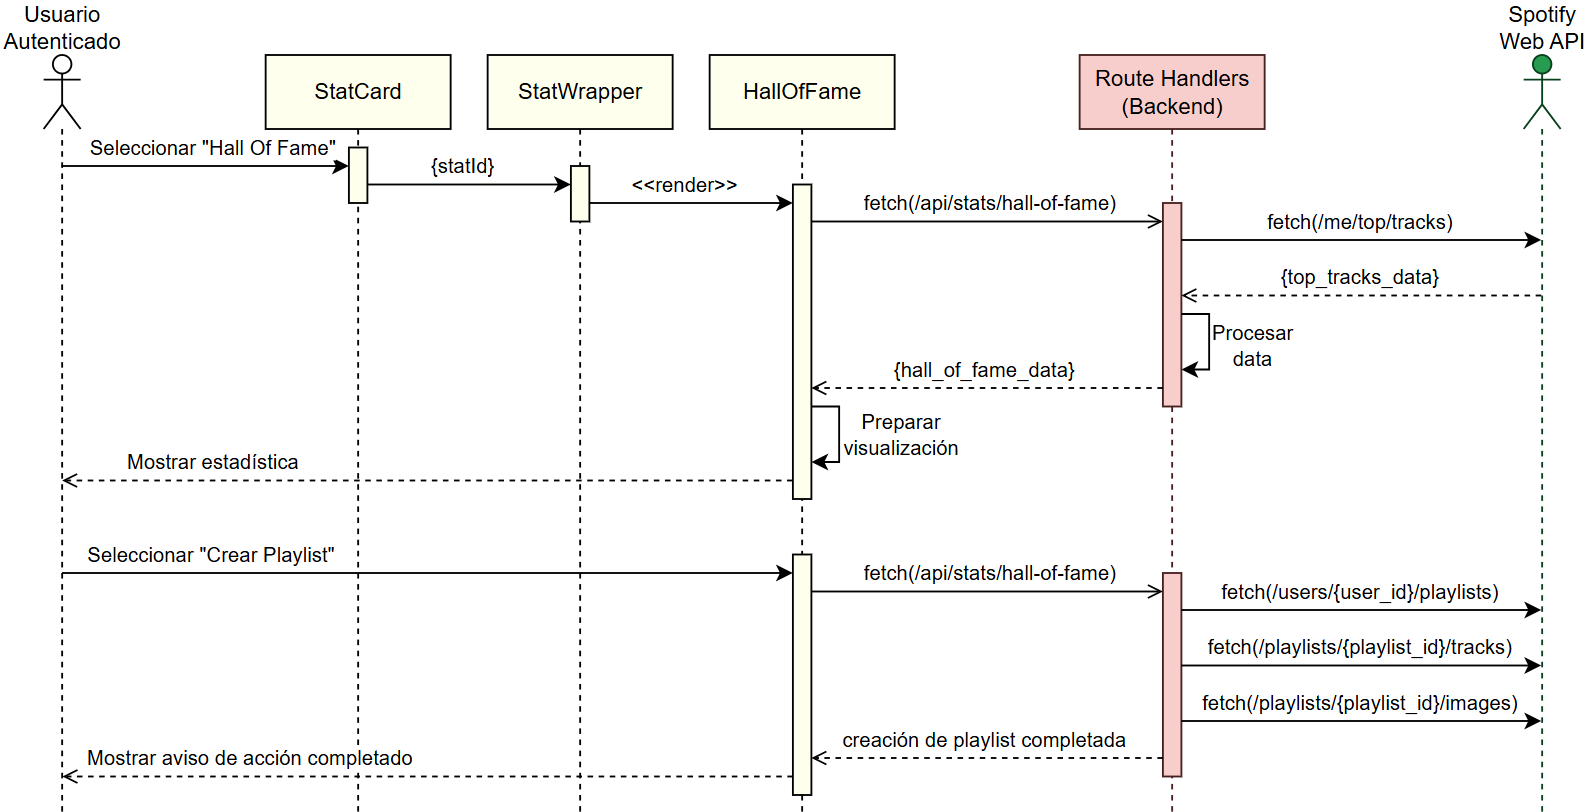
\includegraphics[width=\textwidth]{figures/diagramas_secuencia/ds_ver_hall_of_fame.png}
    \caption{Diagrama de secuencia: Ver Hall Of Fame.}
    \label{fig:ds_ver_hall_of_fame}
\end{figure}

\begin{figure}[H]
    \centering
    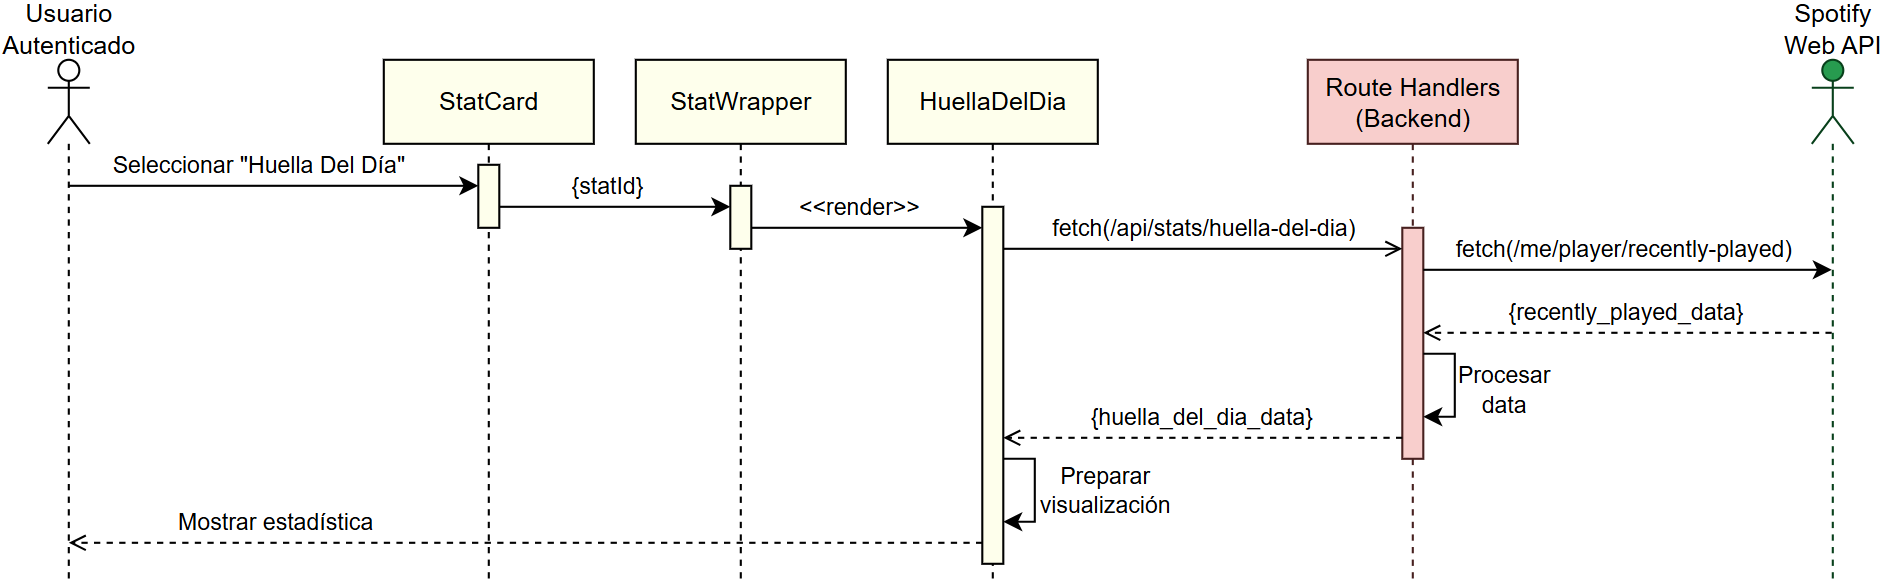
\includegraphics[width=\textwidth]{figures/diagramas_secuencia/ds_ver_huella_del_dia.png}
    \caption{Diagrama de secuencia: Ver Huella Del Día.}
    \label{fig:ds_ver_huella_del_dia}
\end{figure}

\begin{figure}[H]
    \centering
    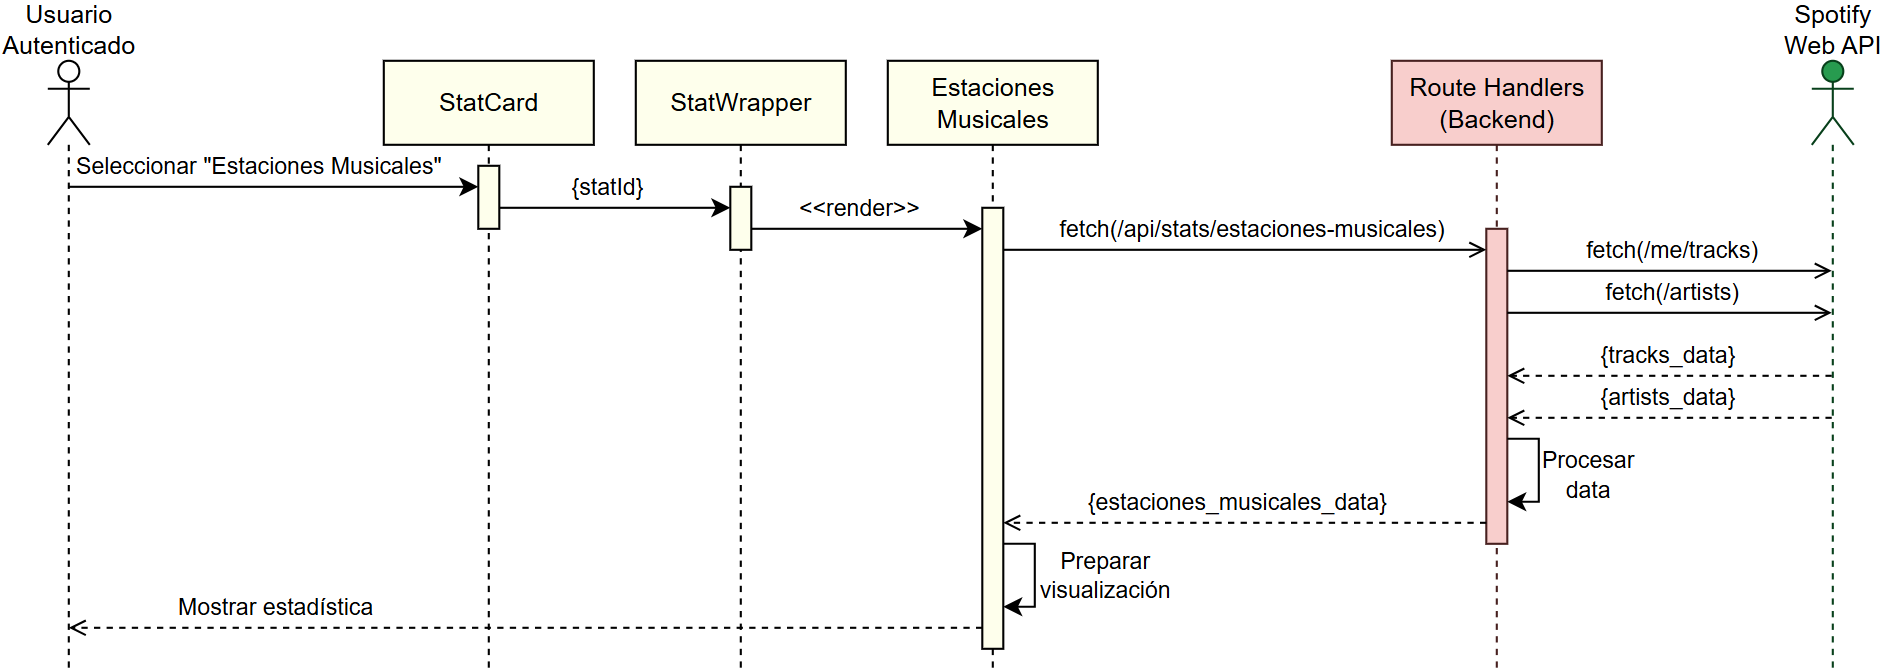
\includegraphics[width=\textwidth]{figures/diagramas_secuencia/ds_ver_estaciones_musicales.png}
    \caption{Diagrama de secuencia: Ver Estaciones Musicales.}
    \label{fig:ds_ver_estaciones_musicales}
\end{figure}

\begin{figure}[H]
    \centering
    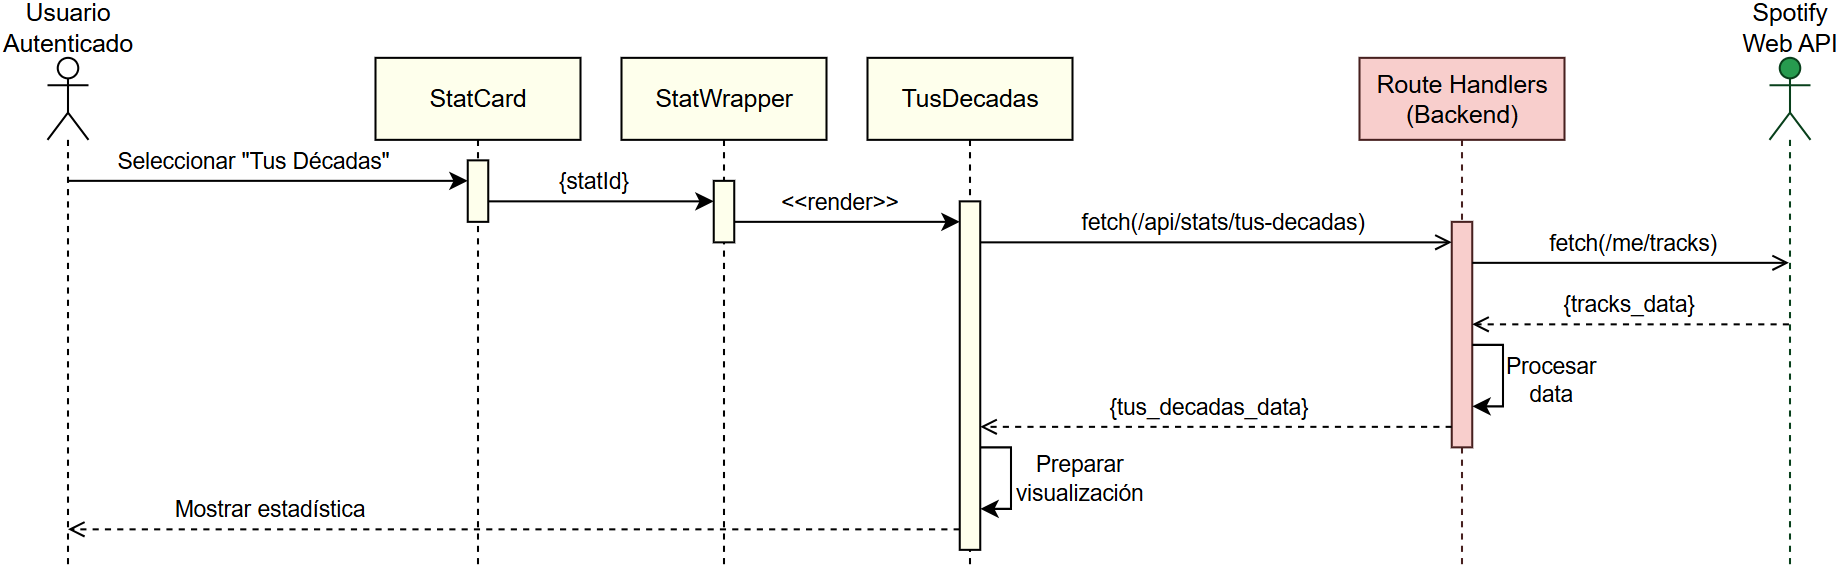
\includegraphics[width=\textwidth]{figures/diagramas_secuencia/ds_ver_tus_decadas.png}
    \caption{Diagrama de secuencia: Ver Tus Décadas.}
    \label{fig:ds_ver_tus_decadas}
\end{figure}

\begin{figure}[H]
    \centering
    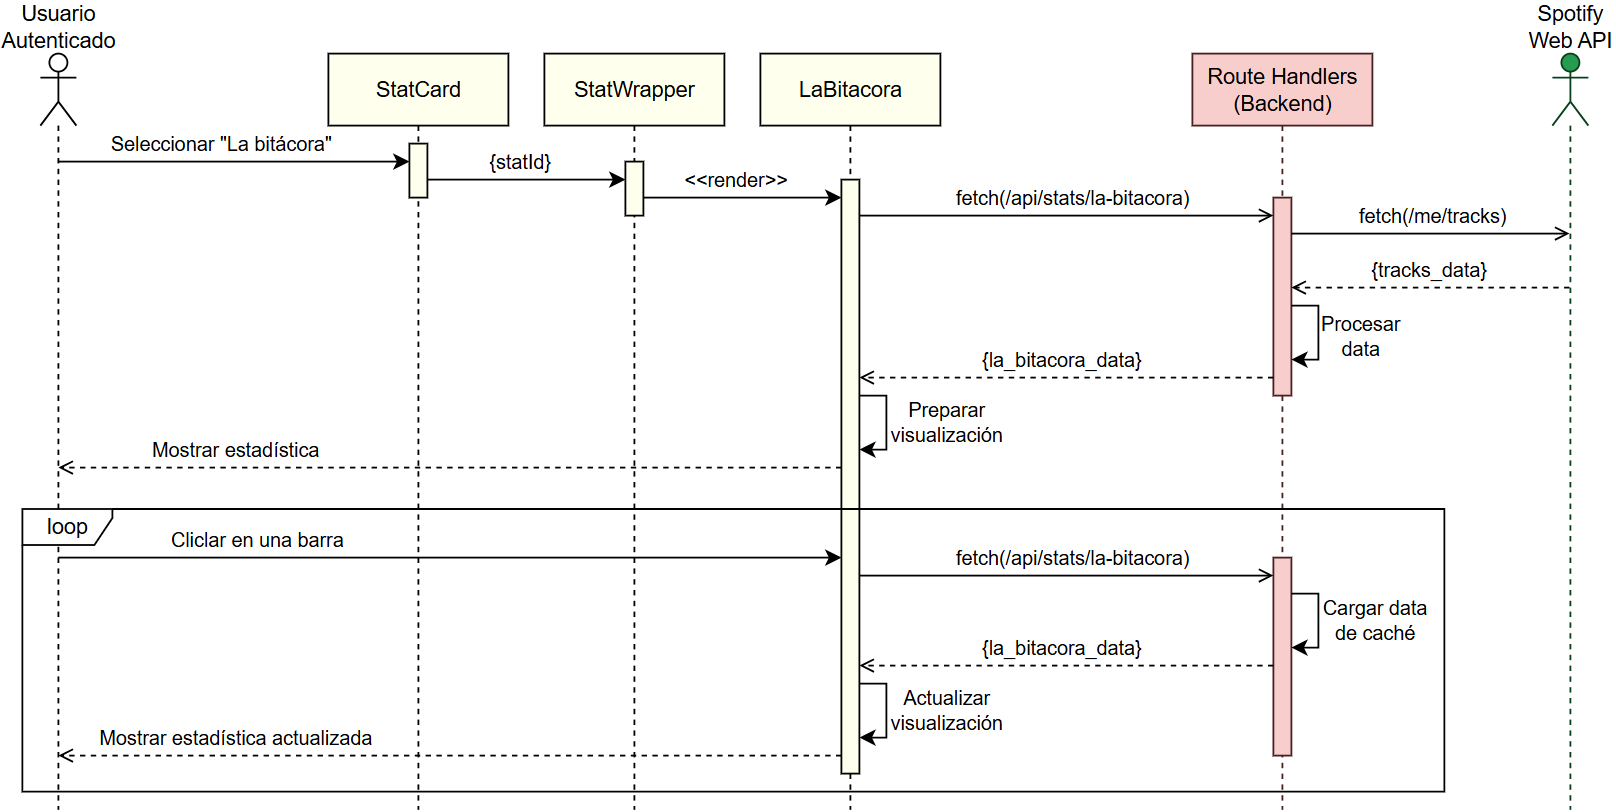
\includegraphics[width=\textwidth]{figures/diagramas_secuencia/ds_ver_la_bitacora.png}
    \caption{Diagrama de secuencia: Ver La Bitácora.}
    \label{fig:ds_ver_la_bitacora}
\end{figure}

\begin{figure}[H]
    \centering
    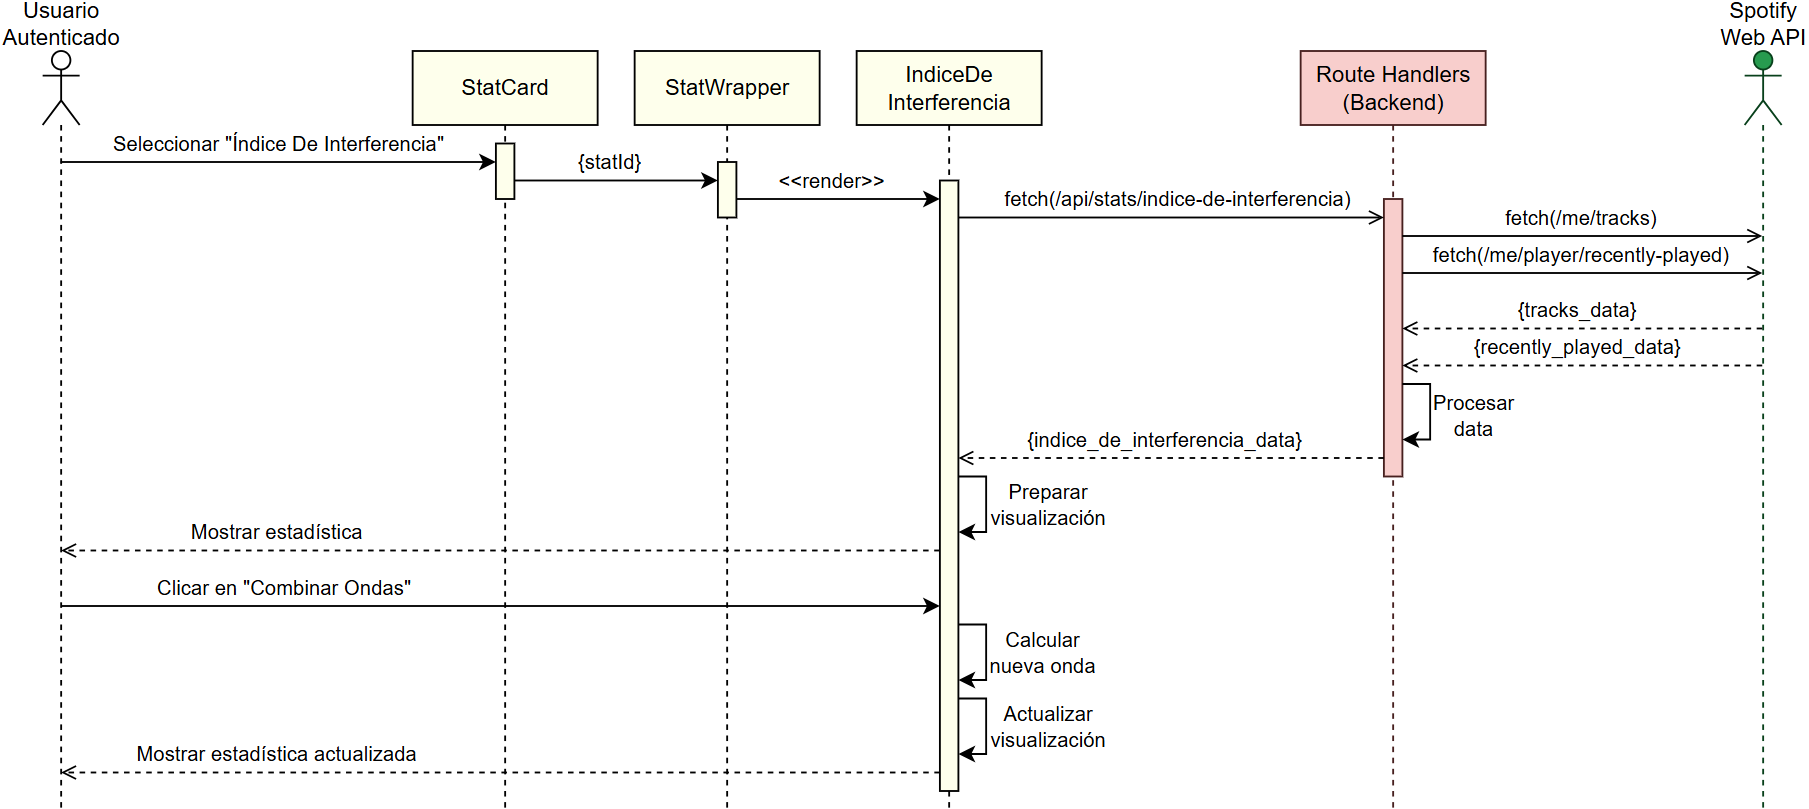
\includegraphics[width=\textwidth]{figures/diagramas_secuencia/ds_ver_indice_de_interferencia.png}
    \caption{Diagrama de secuencia: Ver Índice De Interferencia.}
    \label{fig:ds_ver_indice_de_interferencia}
\end{figure}

\section{Seguridad}

Como esta aplicación maneja información privada de los usuarios, un aspecto crítico en el diseño y desarrollo de la misma es la seguridad. En esta sección se describen las medidas implementadas para proteger los datos de posibles ataques comunes y reducir las vulnerabilidades del sistema.

\subsection{Gestión de Credenciales}

La mala gestión de credenciales es un punto de vulnerabilidad común en aplicaciones web. En el caso del proyecto, se manejan varias credenciales sensibles, especialmente durante el flujo de inicio de sesión. A continuación se detallan las medidas aplicadas a cada una.

\subsubsection*{Client ID y Client Secret}

En la creación de una aplicación que hace uso de la API de \textit{Spotify}, se obtiene un \textbf{client\_id} y un \textbf{client\_secret} que son necesarios para la autenticación con la API. Estas credenciales pertenecen al desarrollador y deben ser protegidas adecuadamente para evitar su exposición a terceros no autorizados. Se almacenan exclusivamente en el servidor, en un archivo de variables de entorno (\texttt{.env.local}), que no se incluye en el control de versiones. En el momento del despliegue, estas variables se cargan en el entorno de producción, que han de ser anteriormente indicadas de manera manual a través de un panel de configuración de \textit{Vercel}. Se puede acceder a estas variables en el lógica del servidor mediante el obtejo \texttt{process.env}.

\subsubsection*{Prevención de CSRF y Scopes}

Para prevenir ataques de \textit{Cross-Site Request Forgery} (CSRF), cada solicitud de inicio de sesión incluye un valor de estado (\textbf{state}) generado de forma aleatoria. Este valor es único para cada sesión y se valida al recibir la respuesta del servidor de autenticación. Este mecanismo, recomendado explícitamente en la documentación de \textit{Spotify} \cite{spotifyAuthCodeFlow2025}, garantiza que las solicitudes sean legítimas y originadas únicamente desde el cliente autorizado, evitando que actores maliciosos puedan ejecutar acciones en nombre del usuario.

Por otro lado, durante el paso de la autorización en el proceso de inicio de sesión, se respeta el principio de mínimos privilegios, donde solo se solicitan los permisos necesarios y ninguno más. Los usuarios son informados claramente sobre los \textbf{scopes} solicitados y su propósito antes de otorgar los permisos. De esta manera se consigue reducir el riesgo de exposición innecesaria de datos.

\subsubsection*{Access Token y Refresh Token}

Una vez que el usuario ha iniciado sesión y la aplicación ha obtenido un \textbf{access\_token} y un \textbf{refresh\_token}, estos se almacenan en unas cookies correspondiente. La configuración de estas cookies es muy importante para protegerlas frente a ataques comunes como \textit{Cross-Site Scripting} (XSS) o \textit{Man-In-The-Middle} (MITM). Las siguientes marcas (\textit{flags}) permiten configurar la seguridad necesaria:

\begin{itemize}
    \item \textbf{\texttt{httpOnly}:} Indicando esta opción como ``\texttt{true}'', asegura que las cookies no puedan ser accedidas por código JavaScript en el navegador, protegiéndolas contra ataques de XSS.
    \item \textbf{\texttt{secure}:} Indicando esta opción como ``\texttt{true}'', las cookies solo pueden ser transmitidas a través de conexiones HTTPS, protegiéndolas contra ataques de MITM. Esta opción solo es necesaria en un entorno de producción, es posible desactivarlo durante el desarrollo.
    \item \textbf{\texttt{maxAge}} Estableciendo un tiempo de vida limitado, se garantiza que se las cookies se eliminen automáticamente una vez cumplido el periodo concretado, minimizando el impacto de un posible compromiso.
\end{itemize}

\subsection{Routing y Conexiones Seguras}

Next.js proporciona un sistema de \textbf{middleware} que permite ejecutar procesos antes de que se manejen las solicitudes de las rutas. En este proyecto, se ha implementado un middleware que verifica la validez de las cookies de sesión antes de permitir el acceso a las rutas protegidas. Si no existe una cookie con un access token, el usuario es redirigido a la página de inicio de sesión, grantizando que solo los usuarios autenticados puedan acceder a las estadísticas y los datos personales.

Para la comunicación entre el cliente y la aplicación, al desplegatse en \textit{Vercel}, éste proporciona automáticamente \textbf{conexiones HTTPS} para todas las solicitudes. Esto garantiza la confidencialidad de los datos transmitidos entre el cliente y el servidor, protegiendo contra ataques de intercepción como el MITM.

\subsection{Otras Medidas}

Del mismo modo que se han implementado mecanismos explícitos para prevenir ataques comunes, la seguridad de una aplicación no solo depende de configuraciones específicas, sino también del entorno de desarrollo y de las prácticas adoptadas a lo largo del ciclo de vida del software. La seguridad implícita, aquella que surge como resultado de buenas prácticas y herramientas adecuadas, desempeña un gran papel.

\begin{itemize}
    \item \textbf{Análisis estático del código con ESLint:} Un linter como \textit{ESLint} permite detectar errores, malas prácticas y patrones potencialmente inseguros en el código TypeScript antes de que lleguen a producción. Integrarlo en el flujo de desarrollo facilita la identificación temprana de vulnerabilidades y la posibilidad de corregirlos antes de que se conviertan en problemas de seguridad.

    \item \textbf{Dependencias actualizadas:} La aplicación se construye sobre versiones recientes y estables de \textit{Next.js}, \textit{React} y \textit{Node.js LTS}, lo que permite beneficiarse de mejoras en seguridad y reducir la exposición a vulnerabilidades conocidas; un riesgo muy común derivado del uso de software obsoleto.

    \item \textbf{Ejecución de pruebas:} Realizar pruebas sistemáticas permite identificar fallos inesperados, comportamientos anómalos o configuraciones incorrectas en la aplicación.

    \item \textbf{Prácticas recomendadas:} Seguir las guías oficiales de seguridad, tanto de la API de \textit{Spotify} como de \textit{Next.js}, garantiza que se cumplen los estándares más recientes.
\end{itemize}

% TODO: Seguir aquí también
\section{Diseño de Pruebas}